\documentclass[letterpaper, 10pt, conference]{ieeeconf}
\usepackage{times}


\IEEEoverridecommandlockouts
\overrideIEEEmargins


\usepackage{cite}
\usepackage{graphicx}
\usepackage{amssymb,amsmath}
\usepackage{algorithm}
\usepackage{color}
\usepackage[noend]{algorithmic}
\usepackage{flushend}
\usepackage[export]{adjustbox}
\renewcommand{\thefootnote}{\fnsymbol{footnote}}

\newcommand{\Acronym}[1]{\ensuremath{{{\texttt{#1}}}}}
\newcommand{\Symbol}[1]{\ensuremath{\mathcal{#1}}}
\newcommand{\Function}[1]{\ensuremath{{ \textsc{#1}}}}
\newcommand{\Constant}[1]{\ensuremath{{\texttt{#1}}}}
\newcommand{\Var}[1]{\ensuremath{{{\textsl{#1}}}}}
\newcommand{\False}{\Constant{false}}
\newcommand{\True}{\Constant{true}}
\newcommand{\Null}{\Constant{null}}
\newcommand{\Name}{\Acronym{dCRoPS}}
\newcommand{\Revision}[1]{\textcolor{red}{#1}}
\newcommand{\R}{\ensuremath{\mathbb{R}}}
\newcommand{\Traj}{\ensuremath{\zeta}}
\newcommand{\Tree}{\Symbol{T}}
\newcommand{\pair}[1]{\ensuremath{\langle#1\rangle}}

\newcommand{\mychange}[1]{\textcolor{red}{#1}}

%\setlength{\abovedisplayskip}{1pt}
%\setlength{\belowdisplayskip}{1pt}

\begin{document}

\title{Path Planning for Swarms in Dynamic Environments by\\ Combining Probabilistic Roadmaps and
  Potential Fields}


\author{Alex Wallar \and Erion Plaku
\thanks{A. Wallar is with the School of Computer Science,
  University of St Andrews, Fife KY16 9AJ, Scotland, UK. E. Plaku is with the
  Dept. of Electrical Engineering and Computer Science, Catholic
  University of America, Washington DC 20064 USA.
}}


\maketitle
\begin{abstract}
This paper presents a path-planning approach to enable a swarm of
robots move to a goal region while avoiding collisions with static and
dynamic obstacles.  To provide scalability and account for the
complexity of the interactions in the swarm, the proposed approach
combines probabilistic roadmaps with potential fields.  The underlying
idea is to provide the swarm with a series of intermediate goals which
are obtained by constructing and searching a roadmap of likely
collision-free guides. As the swarm moves from one intermediate goal
to the next, it relies on potential fields to quickly react and avoid
collisions with static and dynamic obstacles. Potential fields are
also used to ensure that the swarm moves in cohesion. When the swarm
deviates or is unable to reach the planned intermediate goals due to
interferences from the dynamic obstacles, the roadmap is searched again to
provide alternative guides. Experiments conducted in simulation
demonstrate the efficiency and scalability of the approach.
\end{abstract}


\section{Introduction}
\label{sec:Intro}

Emerging applications of swarm robotics in exploration, monitoring,
inspection, and search-and-rescue missions require the swarm to be
able to move to a goal destination while avoiding collisions with
obstacles \cite{swarm,swarmReview12}.  As the swarm is often comprised
of a large number of robots, path planning becomes challenging due to
the high-dimensionality of the underlying configuration space.

As a result, reactive approaches are often employed that avoid
planning directly in the high-dimensional configuration space but
instead regulate the swarm behavior through common rules of
interactions. Stigmergic approaches, inspired by how ants move
back-and-forth from the nest to a food source, utilize synthetic
pheromone traces left in the environment by forager robots to guide
the swarm to the target
\cite{swarmPheromone1,swarmPheromone2,swarmPheromone3}.  While
pheromone-based navigation minimizes communication, it lacks the
flexibility to quickly adapt to dynamic changes in the environment
that could block or disrupt existing pheromone traces. Other
approaches rely on wireless network nodes deployed at various
locations in the environment to provide global coverage and guide the
swarm to the target \cite{swarmComm1,swarmComm2}.  Genetic algorithms
have also been used to facilitate navigation by evolving collective
behaviors for the swarm, such as chain formation or obstacle avoidance
\cite{swarmEvolve1,swarmEvolve2}.  In leader-follower approaches, one
or few robots move along precomputed paths to the target location
while the rest of the swarm seeks to follow the leaders, often
maintaining a desired formation
\cite{swarmLeader1,swarmLeader2,swarmLeader3}. The work in
\cite{JurVel} proposes a fully-decentralized algorithm based on
the concept of reciprocal velocity obstacles to enable collision-free
motions among a group of robots. Other approaches based
on virtual fixtures treat the swarm as a rigid body, seeking to
maintain a fixed relation among swarm members
\cite{swarmFixture1,swarmFixture2,swarmFixture3}. While such
approaches reduce swarm path planning to single-robot planning, the
imposed structure rigidity and the increased dimensionality make it
difficult to efficiently plan paths especially when considering a
large number of robots.


Artificial potential functions (APFs) provide a common approach for
swarm path planning by imposing virtual repulsive forces from
obstacles and attractive forces to the goal
\cite{Khatib86,reif1999social,book:SwarmsAPFs,tanner2005formation,swarmPF1,swarmPF2}.
APFs are fast to compute as the resulting forces for each robot in the
swarm depend only on the nearby obstacles, the goal region, and
limited interactions with neighboring robots in the swarm.  While APFs
provide local, reactive, behaviors that enable the swarm to avoid
obstacles, the global path guidance toward the goal suffers from local
minima.  This limitation of APFs becomes more prevalent when
considering path planning for large swarms moving in cluttered
environments. Designing APFs that avoid or minimize the likelihood of
the robots becoming stuck in local minima remains a challenging problem
\cite{RK92}.

Alternative approaches seek to avoid local minima by relying on global
path planning. Probabilistic roadmaps (PRM) \cite{PRM} and other
sampling-based path planners
\cite{RRT,RRTRecent1,TogglePRM,UOBPRM,PlakuTRO10} provide global path
planning by using sampling to capture the connectivity of the free
configuration space. In particular, PRM approaches construct roadmaps
resembling a network of roads obtained by sampling a large number of
configurations and connecting neighboring configurations via
collision-free paths.  The roadmap is then used to perform different
tasks, such as homing, goal searching, or shepherding
\cite{LienSwarming,LienShepherding}.  PRMs have also been combined
with Bezier curves to guide a number of nonholonomic robots to the
goal while maintaining formation \cite{KostasSwarm}.

While PRMs avoids the issues associated with local minima, scalability
starts becoming problematic when dealing with a large number of
robots. As the configuration space of a swarm consist of the Cartesian
product of the individual configuration spaces of each robot, it
becomes challenging to generate collision-free configurations and
connect neighboring configurations via collision-free paths.

To provide scalability and account for the complexity of the
interactions in the swarm, this paper builds upon our prior work
\cite{PlakuTAROS13boids} which combined PRMs with APFs. While prior
work was limited to static obstacles, the proposed approach, termed
$\Name$ (\texttt{C}ombined \texttt{Ro}admaps and \texttt{P}otentials
for \texttt{S}warms for \texttt{D}ynamic Obstacles), can efficiently
guide the swarm to the goal even in the presence of dynamic obstacles.
The underlying idea is to provide the swarm with a series of
intermediate goals which are obtained by constructing and searching a
roadmap of likely collision-free guides. To maintain scalability, the
roadmap is constructed over the two-dimensional workspace in which the
swarm moves rather than the high-dimensional configuration space
associated with the swarm. As the swarm moves from one intermediate
goal to the next, it relies on potential fields to quickly react and
avoid collisions with static and dynamic obstacles.  


In contrast to prior work \cite{PlakuTAROS13boids}, $\Name$ provides
robots in the swarm with alternative guides to the goal when a robot
is unable to reach the planned intermediate targets due to
interferences from the dynamic obstacles. Weights of roadmap edges in
or near the obstructed area are dynamically adjusted to account for
lack of progress and to guide the swarm away from such areas.  While
it may also be possible to use grids or Voronoi diagrams to guide the
swarm, roadmaps have been shown to better capture the connectivity of
the free space \cite{book:MP}[chap.~7]. %Moreover, guides over grids or
%Voronoi diagrams would have a particular, regular, structure which is
%generally not suitable for the complex environments considered in this
%paper. In contrast, roadmaps, due to the probabilistic sampling, are
%able to provide the swarm with many different alternative guides to
%the goal region.
 
$\Name$ also improves the APFs over our prior work
\cite{PlakuTAROS13boids} in order to enable the swarm to react rapidly
to the dynamic obstacles moving towards it.  In particular, $\Name$
introduces a potential field which influences the heading of a robot
$b$ by leveraging the headings of other robots that have been in the
past close to $b$'s current position and have managed to make further
progress toward the goal.


Experiments are conducted in
simulation where large swarms have to move in complex environments,
often through narrow passages, while avoiding collisions with static
obstacles and numerous dynamic obstacles. Results demonstrate the
efficiency and scalability of $\Name$.

\section{Problem Formulation}
\label{sec:Problem}
The swarm consists of a number of mobile circular robots
$b_1, \ldots, b_m$. The swarm operates inside a
two-dimensional environment $W$ populated by polygonal static and
dynamic obstacles, denoted as $\Var{StaticObstacles}$ and
$\Var{DynamicObstacles}$, respectively.  While the static obstacles
remain fixed, the dynamic obstacles move along different directions.
Starting at an initial placement, the objective is for each robot to
reach a goal region $G \subset W$ while avoiding collisions with the
static and dynamic obstacles in $W$.


Each robot is capable of detecting nearby obstacles within
$\Delta_\Var{obst}$ radius. $\Name$ seeks to keep the robots moving as
one group as much as possible, separating into two or more groups only
when necessary to avoid the dynamic obstacles.  The geometry and
placement of each static obstacle is assumed to be available
beforehand. No information is given to $\Name$ beforehand in regards
to the dynamic obstacles.  In the experiments, the dynamic obstacles
move along random directions, which are not known to $\Name$.


\section{Method}
\label{sec:Method}

Pseudocode for $\Name$ is provided in Alg.~\ref{algo}. The
main steps are described below.


\subsection{Global Path Planning}

$\Name$ uses a roadmap to provide each robot in the swarm with global
path planning and find alternative guides to the goal region when dynamic
obstacles prevent a robot from moving along its current guide.

\subsubsection{Roadmap Construction}
\label{sec:RoadmapConstruction}
Pseudocode for the roadmap construction is provided in Alg.~\ref{algo:PRM}.
The roadmap is represented as a graph $RM=(V,E)$. A vertex $q \in V$
corresponds to a collision-free point in $W$. An edge
$(q_i, q_j) \in E$ corresponds to a collision-free straight-line
segment from $q_i$ to $q_j$.  Collision checking during roadmap
construction is performed with respect to the static obstacles, which
are assumed to be known.

%Each roadmap vertex is generated by repeatedly sampling a point at random
%inside $W$ until it is a certain distance \mychange{Can you rephrase this, it
%does not sound clear}, $d_\Var{clear}$, away from the static
%obstacles.  

To generate a roadmap vertex, a point is sampled uniformly at random
inside $W$. The point is checked whether it is at least a certain
distance, $d_\Var{clear}$, away from the static obstacles. If so, the
sampled point is added as a roadmap vertex. Otherwise, this sampling
process is repeated until the sampled point has a clearance of
$d_\Var{clear}$ from the static obstacles (Alg.~\ref{algo:PRM}:1--4).
In this way, $\Name$ seeks to avoid areas close to the obstacles since
such areas are more likely to lead to collisions with the dynamic
obstacles, other robots, and static obstacles.  The total number of
roadmap vertices, $n$, is provided by the user.  This is a common
strategy in PRM approaches \cite{PRM,book:MP}, as it is difficult to
determine beforehand an optimal number of roadmap vertices
\cite{IncrementalPRM}.  Experiments are presented in
Section~\ref{sec:ExpResults} that show the impact of the roadmap size
on the overall performance of $\Name$.

%A weight $w(q)$ is associated with each vertex $q \in V$ as an
%estimate on the feasibility of the swarm to pass near $q$. More
%specifically, $w(q)$ is defined as
%$$
%w(q) = (\sum_{o \in \Var{StaticObstacles}} \Var{dist}(q, o))^3,
%$$
%where $\Var{dist}(q, o)$ denotes the distance from the point $q$ to
%the obstacle $o$. Small values of $w(q)$ are indicative of nearby
%obstacles, which the swarm will seek to avoid.
%Note that while we have chosen
%through experimentation a particular definition of $w(q)$ for this
%paper, alternative weight functions can also be used.

Roadmap edges are generated by connecting each $q \in V$ with
straight-line segments to its $k$-nearest roadmap vertices according
to the Euclidean distance (Alg.~\ref{algo:PRM}:6--7). Collision
checking is performed with respect to the static obstacles, discarding
any edge that is found in collision (Alg.~\ref{algo:PRM}:8). A weight
$w(q_i, q_j)$ is associated with each edge $(q_i, q_j) \in E$ as an
estimate on the feasibility of having the swarm move from $q_i$ to
$q_j$ (Alg.~\ref{algo:PRM}:9). More specifically, $w(q_i, q_j)$ is defined as
$$
w(q_i, q_j) = \left(\min_{o \in \Var{StaticObstacles}} \Var{dist}((q_i,
q_j), o)\right)^{-3},
$$ where $\Var{dist}((q_i, q_j), o)$ denotes the Euclidean distance
between the static obstacle $o$ and the straight-line segment from
$q_i$ to $q_j$.  As such, small values of $w(q_i, q_j)$ indicate that
the straight-line segment from $q_i$ to $q_j$ is away from the static
obstacles. As explained later, $\Name$ guides the swarm along
low-weight roadmap edges in order to make it easier to avoid collisions with
the static and dynamic obstacles, and to minimize congestion within
the swarm.  Note that while we have chosen through experimentation a
particular definition of $w(q_i, q_j)$ for this paper, alternative weight
functions can also be used.

\begin{algorithm}[t]
\caption{Pseudocode for $\Name$}
\label{algo}
{\small{
\begin{algorithmic}[1]
\setcounter{ALC@line}{0}
%\COMMENT{generate $n$ additional roadmap vertices}
\vspace*{1mm}

\STATE $\pair{RM = (V, E), w} \leftarrow \Function{roadmap}(W, n, k, d_\Var{clear})$

\FOR{$b \in \Var{Robots}$}
\STATE $b.\Var{guide} \leftarrow \emptyset$;
       $b.\Var{finalGoal} \leftarrow \Function{RandomPoint}(G)$
\ENDFOR
\WHILE{$\exists b \in \Var{Robots}$ \textbf{with} $b.\Var{pos} \not\in
  G$}
\FOR{$o \in \Var{DynamicObstacles}$}
\STATE  $o.\Var{pos} \leftarrow \Function{MoveDynamicObstacle}(o)$
\ENDFOR
\FOR{$b \in \Var{Robots}$ \textbf{with} $b.\Var{pos} \not\in G$}
\IF{$b.\Var{guide} = \emptyset$}
\STATE $b.\Var{guide} \leftarrow \Function{guide}(RM, w, b.\Var{pos}, b.\Var{finalGoal})$
\STATE $b.\Var{next} \leftarrow 1$
\ENDIF
\STATE \textbf{while} {$||b.\Var{pos},
  b.\Var{guide}(b.\Var{next}||_2 \leq d_\Var{reach}$\\ \textbf{and}
 $b.\Var{next} < |b.\Var{guide}|$}
\textbf{do} $b.\Var{next} \leftarrow b.\Var{next} + 1$

\STATE $b.\Var{heading} \leftarrow \Function{superimpose}(PF_\Var{obst}(b),
PF_\Var{sep}(b),$\\ \hfill{$PF_\Var{next}(b),PF_\Var{hist}(b))$}
%\STATE $b.\Var{pos} \leftarrow b.\Var{pos} + \Var{step} \frac{(v_x,
%  v_y)}{||(v_x, v_y)||_2}$
\STATE $b.\Var{pos} \leftarrow b.\Var{pos} + \Var{step} \cdot \frac{b.\Var{heading}}
{||b.\Var{heading}||_2}$
\STATE \textbf{if} $\Function{collision}(b)$ \textbf{return} \Constant{failure}
\COMMENT{compute alternative guide if necessary}
\IF{$\Function{stuck}(b) = \True$}
\FOR{$\ell = b.\Var{next} \ldots \min(b.\Var{next} + \Var{e},  |b.\Var{guide}| - 1)$}
\STATE $q_i \leftarrow b.\Var{guide}(\ell)$; $q_j \leftarrow
b.\Var{guide}(\ell + 1)$
\STATE $w(q_i, q_j) \leftarrow w(q_i, q_j) \cdot \Var{penalty}$
\ENDFOR
\STATE $b.\Var{finalGoal} \leftarrow \Function{RandomPoint}(G)$
\STATE $b.\Var{guide} \leftarrow \Function{guide}(RM, w, b.\Var{pos}, b.\Var{finalGoal})$
\ENDIF
\ENDFOR
\ENDWHILE
\STATE \textbf{return} \Constant{success}


\end{algorithmic}
}}
\end{algorithm}


\begin{algorithm}[t]
\caption{$\Function{roadmap}(W, n, k, d_\Var{clear})$}
\label{algo:PRM}
{\small{
\begin{algorithmic}[1]
\setcounter{ALC@line}{0}
%\COMMENT{generate $n$ additional roadmap vertices}
\vspace*{1mm}

%\FOR{$b \in \Var{Robots}$}
%\STATE $b.\Var{goalPos} \leftarrow \Function{RandomPoint}(G)$; $V \leftarrow V \cup \{b.\Var{goalPos}\}$
%\ENDFOR
\FOR{$i = 1 \ldots n$}
\STATE \textbf{repeat} $q \leftarrow \Function{RandomPoint}(W)$
\STATE \textbf{until} {$\left(\min_{o \in \Var{StaticObstacles}}\Var{dist}(q,
  o)\right) > d_\Var{clear}$}
\STATE $V \leftarrow V \cup \{q\}$
\ENDFOR
\FOR{$q_i \in V$}
\FOR{$q_j \in \Function{neighs}(V, q_i, k)$}
\IF{$\Function{collision}(q_i, q_j, \Var{StaticObstacles}) = \False$}
\STATE $E \leftarrow E \cup \{(q_i, q_j)\}$
\STATE $w(q_i, q_j) \leftarrow
\left(\min_{o\in\Var{StaticObstacles}} \Var{dist}((q_i, q_j), o)\right)^{-3}$
\ENDIF
\ENDFOR
\ENDFOR
\STATE \textbf{return} $(RM=(V,E), w)$
\end{algorithmic}
}}
\end{algorithm}


\begin{figure}
{\footnotesize{
\begin{tabular}{r|ll}
param & description \hfill{section} \\\hline
$n$ & number of roadmap vertices   \hfill{\S\ref{sec:RoadmapConstruction}}\\
$k$ & number of nearest neighbors in roadmap  \hfill{\S\ref{sec:RoadmapConstruction}}\\
$d_\Var{clear}$ & clearance from static obstacles  \hfill{\S\ref{sec:RoadmapConstruction}}\\
$d_\Var{reach}$ & next target radius  \hfill{\S\ref{sec:Guide}}\\
$\Var{step}$ & robot step size\hfill{\S\ref{sec:Guide}} \\
$e$ & number of current guide edges to penalize  \hfill{\S\ref{sec:Branching}}\\
$\Var{penalty}$ & scaling factor for current guide edges   \hfill{\S\ref{sec:Branching}}\\
$\delta_\Var{next}$ & scaling constant for $PF_\Var{next}$  \hfill{\S\ref{sec:PFnext}} \\
$\delta_\Var{obst}$ & scaling constant for $PF_\Var{obst}$  \hfill{\S\ref{sec:PFobst}} \\
$\Delta_\Var{obst}$ & radius of influence for $PF_\Var{obst}$ \hfill{\S\ref{sec:PFobst}}\\
$\delta_\Var{sep}$ & scaling constant for $PF_\Var{sep}$  \hfill{\S\ref{sec:PFsep}}\\
$\Delta_\Var{sep}$ & radius of influence for $PF_\Var{sep}$  \hfill{\S\ref{sec:PFsep}}\\
$\delta_\Var{hist}$ & scaling constant for $PF_\Var{hist}$  \hfill{\S\ref{sec:PFhist}}\\
\end{tabular}
}}
\caption{Parameters used by $\Name$. More details can be found in the
  corresponding sections.}
\label{table:Params}
\end{figure}

\subsubsection{Guiding the Swarm}
\label{sec:Guide}

In order to move the swarm toward the goal region $G$, each robot $b
\in \Var{Robots}$ is provided with a global guide, denoted by
$b.\Var{guide}$, which represents a path along low-weight roadmap edges
from the current position of the robot, denoted by $b.\Var{pos}$,  to
the goal region $G$. More precisely, each
robot $b$ is initially assigned a random point inside $G$ to act as
its final goal, denoted by $b.\Var{finalGoal}$ (Alg.~\ref{algo}:3).
Then, $b.\Var{guide}$ is computed as the shortest path in the roadmap
$RM = (V, E)$ from $q'$ to $q''$, where $q'$ is the closest roadmap
vertex to $b.\Var{pos}$ and $q''$ is the closest roadmap vertex to
$b.\Var{finalGoal}$ (Alg.~\ref{algo}:9). A* search is used to make the
computation of the guide efficient. 

Each robot $b$ then seeks to reach $G$ by following its guide, i.e.,
going to $b.\Var{guide}(1), \ldots, b.\Var{guide}(|b.\Var{guide}|)$ in
succession. More precisely, $b.\Var{next}$ keeps track of the index in
$b.\Var{guide}$ which serves as the next target for $b$. Initially,
$b.\Var{next}$ is set to $1$ since $b$ seeks to move to
$b.\Var{guide}(1)$ (Alg.~\ref{algo}:10). The target is considered to
be reached when $b.\Var{pos}$ is within a certain radius,
$d_\Var{reach}$, from $b.\Var{guide}(b.\Var{next})$.  When $b$ reaches
$b.\Var{guide}(1)$, then $b.\Var{next}$ is set to $2$, and so on
(Alg.~\ref{algo}:11).  

As discussed later in Section~\ref{sec:Local}, potential fields are
used to move $b$ from its current position to the next target
$b.\Var{guide}(b.\Var{next})$.  The combination of these potential
fields determines the vector $b.\Var{heading}$ along which the robot
$b$ should move in order to make progress toward the next target,
$b.\Var{guide}(b.\Var{next})$, while avoiding collisions with the
dynamic obstacles, static obstacles, and other robots. The robot $b$
then takes a step along this direction (Alg.~\ref{algo}:12--13).


\subsubsection{Global Replanning via Alternative Guides}
\label{sec:Branching}
If a robot $b$ gets stuck in a local minima or a dynamic obstacle
prevents it from reaching its next target
$b.\Var{guide}(b.\Var{next})$ along its current guide, $\Name$ will
search the roadmap again to find an alternative guide for $b$
(Alg.~\ref{algo}:15--19). This is akin to the replanning stage used in
sampling-based motion planning
\cite{van2006anytime,ferguson2006anytime,karaman2011anytime}.  Before
the roadmap search, $\Name$ adjusts the weight of the next few edges
on the current guide in order to guide $b$ away from this area.  More
precisely, let $q(i) = b.\Var{guide}(b.\Var{next} + i)$. Then, $\Name$
scales the weight of edges $(q(0), q(1)), \ldots, (q(\Var{e} - 1),
q(\Var{e}))$ by a factor $\Var{penalize} > 1$,
where $e$ is the number of edges to penalize. As a result of these
weight increases, the shortest-path search will produce an alternative
guide.

 This adjustment of edge weights is used to relieve swarm congestion
 when it is confronted by an obstructing obstacle. The creation of a
 new guide provides the robot with an alternative pathway, which could
 help it reduce the average wait time, the average time stuck, and it
 can guide the swarm around obstructing dynamic obstacles that are
 blocking critical passageways.

\subsection{Local Path Planning}
\label{sec:Local}

$\Name$ uses APFs to make each robot in the swarm follow its
guide and quickly react to obstacles it may encounter along the way.
Several criteria are taken into consideration when designing
the APFs for a robot $b$:
\begin{enumerate}
\item $b$ is attracted to its next target $b.\Var{guide}(b.\Var{next})$;
\item $b$ is repulsed away from obstacles;
\item $b$ moves in cohesion with the other robots while maintaining some separation from neighboring robots in order
  to minimize the risk of robot-robot collisions;
\item $b$ leverages the headings of
other robots that have been in the past close to $b$'s current position and have
managed to make further progress.
\end{enumerate}

\subsubsection{Attraction to the Next Target along the Current Guide}
\label{sec:PFnext}
To pull the
robot to the next target, $\Name$ defines an attractive potential as follows:
\begin{eqnarray*}
PF_\Var{next}(b) &=&  
\delta_\Var{next}\cdot (b.\Var{guide}(b.\Var{next}) - b.\Var{pos}) \cdot \\
& & ||b.\Var{guide}(b.\Var{next}) - b.\Var{pos}||_2,
\end{eqnarray*}
where $\delta_\Var{next}$ is a scaling constant. Note that when the
robot is away from its next target, the potential exerts a larger
attractive force to bring the robot closer.


\subsubsection{Repulsion from Obstacles}
\label{sec:PFobst}
To avoid collisions, $\Name$ relies on a repulsive potential to push
each robot away from the obstacles. Since $\Name$ is
designed for dynamic obstacles, the responsiveness in the
obstacle potential needs to also increase in order for the
robots to react quickly to moving obstacles. More specifically,
the repulsive potential between a robot $b$ and an obstacle $o$ is
defined as
$$
PF_\Var{obst}(b, o) = \delta_\Var{obst} \frac{b.\Var{pos}
- \Var{ClosestPoint}(o, b.\Var{pos})}{(\Var{dist}(b.\Var{pos}, o))^2},
$$
where $\delta_\Var{obst}$ is a scaling constant and
$\Var{dist}(b.\Var{pos}, o)$ is the distance from the point
$b.\Var{pos}$ to the obstacle $o$.
As it is common in APFs, obstacles that are far away do not exert any
repulsive forces. As such, only obstacles that are within a certain
distance $\Delta_\Var{obst}$ from $\Var{pos}_b$ are used for the
computation of the overall repulsive potential, i.e.,
$$
PF_\Var{obst}(b) = \sum_{\stackrel{o \in
    \Var{StaticObstacles} \cup \Var{DynamicObstacles}}{\Var{dist}(b.\Var{pos}, o) \leq \Delta_\Var{obst}}}  PF_\Var{obst}(b, o).
$$

\subsubsection{Repulsion from Neighboring Robots}
\label{sec:PFsep}
In order to ensure that robots do not get too close to one another,
which could lead to collisions and swarm congestion, $\Name$ imposes a
repulsive potential. A weak potential is used instead of a strong one
as the objective is to push $b$ at a safe distance from its neighbors
but not to separate it from the swarm. For this reason, the repulsive
potential between two robots $b_i$ and $b_j$ is defined as
$$
PF_\Var{sep}(b_i, b_j) = \delta_\Var{sep} \frac{b_i.\Var{pos}-b_j.\Var{pos}}{
||b_i.\Var{pos}, b_j.\Var{pos}_{b_j}||_2},
$$
where $\delta_\Var{sep}$ is a scaling constant. Similar to the case of
the repulsive potential for obstacles, only robots that are within a
certain distance $\Delta_\Var{sep}$ have an influence on $b$, i.e.,
$$
PF_\Var{sep}(b) = \sum_{\stackrel{b_i \in
    \Var{Robots} - \{b\}}{\Var{dist}(b, b_i) \leq \Delta_\Var{sep}}}  PF_\Var{sep}(b, b_i).
$$

\subsubsection{Leveraging History}
\label{sec:PFhist}
The heading of the robot $b$ is also influenced by the headings of
other robots that have been in the past close to $b$'s current position and have
managed to make further progress. More specifically, a grid is
implicitly imposed on $W$. Each grid cell $c$ keeps track of the
heading of the robots that have entered $c$ in the past and have then
left it -- the list of such robots is denoted by $c.\Var{Robots}$.
Then,
$$
PF_\Var{hist}(b) = \frac{\delta_\Var{hist}}{|\Var{cell}(b).\Var{Robots}|}\sum_{b' \in \Var{cell}(b).\Var{Robots}} b'.\Var{lastHeading},
$$ where $\delta_\Var{hist}$ is a scaling constant, $\Var{cell}(b)$
denotes the grid cell that contains $b.\Var{pos}$, and
$b'.\Var{lastHeading}$ denotes the direction of $b'$ when it was last
in $\Var{cell}(b)$. In this way, $b$ can use the heading of other
robots that have left $\Var{cell}(b)$ so that it too can leave this
cell and make progress toward the next target. By following headings
of other robots, this potential field also promotes cohesion among
robots in the swarm.


\subsubsection{Combining the Potential Fields}
\label{sec:PFcombine}
The overall effect on $b$ is obtained by combining the four different
potential fields:
$$
PF(b) = \frac{\sum_{\phi \in \Var{fields}} \left(|| PF_\phi(b)||_2
  PF_\phi(b)\right)}{\sum_{\phi \in \Var{fields}} || PF_\phi(b)||_2},
$$ where $\Var{fields} = \{\Var{next}, \Var{obst}, \Var{sep},
\Var{hist}\}$. This overall force is then used to update the heading
and position of $b$ (Alg.~\ref{algo}:12--13).  In this way, $b$ is
attracted to the next target, strongly repulsed from the obstacles,
seeks to maintain a separation distance from its neighbors, and
leverages headings of other robots to move to the next target. When a
robot becomes stuck, the weights associated with the next several
roadmap edges of the guide are increased, and a new alternative guide
is computed to help it escape.  This combination of global path
planning via roadmaps and local path planning via potential fields
enables the approach to effectively guide the swarm to the final goal
while avoiding collisions with the static and dynamic obstacles.


\section{Experiments and Results}
\label{sec:ExpResults}

Experiments are conducted in simulation with an increasing number of
robots moving in complex environments, seeking to avoid numerous
static and dynamic obstacles. The scene models and parameter values used in the
experiments are made publicly available \cite{dCrops}.

\begin{figure}
\centering
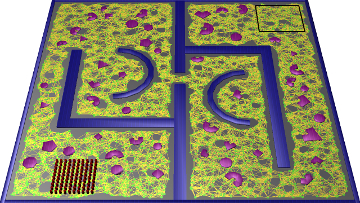
\includegraphics[width=\columnwidth]{usef/figA_PRM_scaled.jpg}\\
(a) scene 1 \\
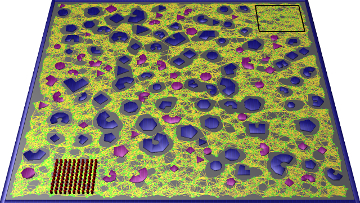
\includegraphics[width=\columnwidth]{usef/figB_PRM_scaled.jpg}\\
(b) scene 2 \\
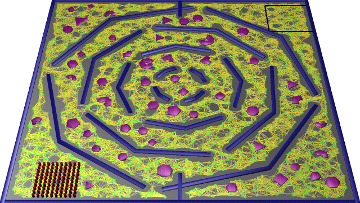
\includegraphics[width=\columnwidth]{usef/figC_PRM_scaled.jpg} \\
(c) scene 3
\caption{Scenes used for the experiments. Each figure shows the static
  obstacles (blue), initial placement of the dynamic obstacles (magenta), initial placement of
  the robots (red), goal region (black box), and the roadmap (roadmap
  vertices are shown as green circle and roadmap edges are shown as
  yellow segments). Recall that collision checking in the roadmap is
  done only with respect to the static obstacles which are known
  beforehand.}
\label{fig:Scenes}
\end{figure}

\begin{figure*}
\centering
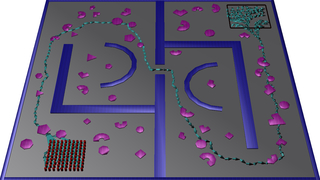
\includegraphics[width=0.24\textwidth]{usef/figA_Inter1_scaled.jpg}
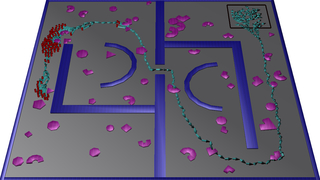
\includegraphics[width=0.24\textwidth]{usef/figA_Inter2_scaled.jpg}
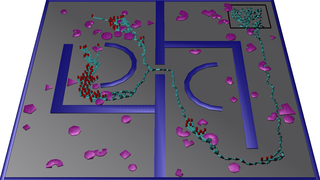
\includegraphics[width=0.24\textwidth]{usef/figA_Inter3_scaled.jpg}
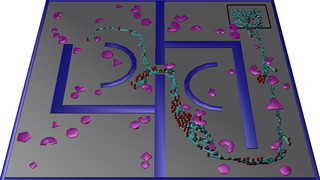
\includegraphics[width=0.24\textwidth]{usef/figA_Inter4_scaled.jpg}\\[2mm]
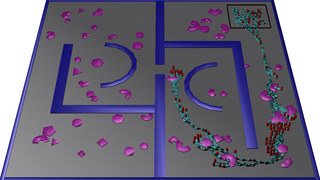
\includegraphics[width=0.24\textwidth]{usef/figA_Inter5_scaled.jpg}
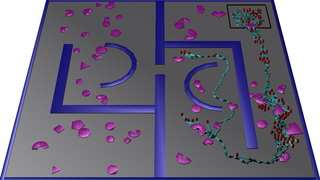
\includegraphics[width=0.24\textwidth]{usef/figA_Inter6_scaled.jpg}
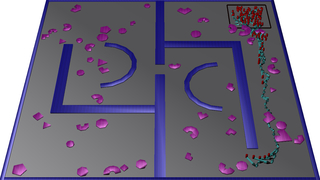
\includegraphics[width=0.24\textwidth]{usef/figA_Inter7_scaled.jpg}
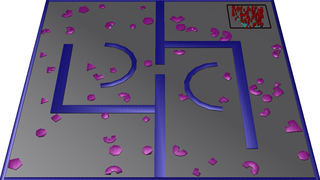
\includegraphics[width=0.24\textwidth]{usef/figA_Inter8_scaled.jpg}\\[2mm]
(a) scene 1\\[2mm]
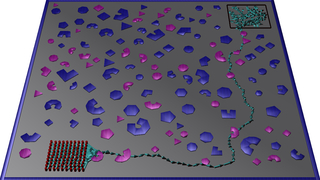
\includegraphics[width=0.24\textwidth]{usef/figB_Inter1_scaled.jpg}
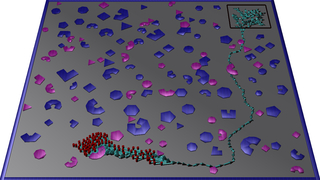
\includegraphics[width=0.24\textwidth]{usef/figB_Inter2_scaled.jpg}
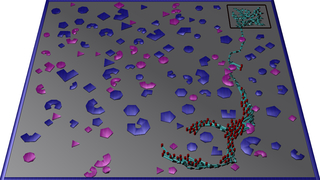
\includegraphics[width=0.24\textwidth]{usef/figB_Inter3_scaled.jpg}
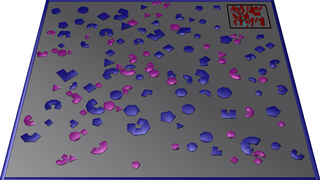
\includegraphics[width=0.24\textwidth]{usef/figB_Inter4_scaled.jpg}\\[2mm]

(b) scene 2\\[2mm]
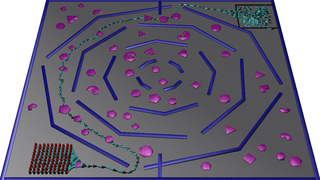
\includegraphics[width=0.24\textwidth]{usef/figC_Inter1_scaled.jpg}
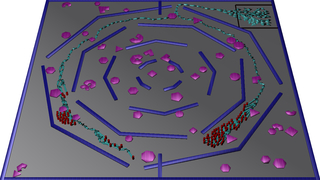
\includegraphics[width=0.24\textwidth]{usef/figC_Inter2_scaled.jpg}
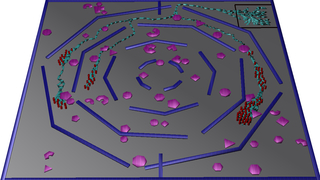
\includegraphics[width=0.24\textwidth]{usef/figC_Inter3_scaled.jpg}
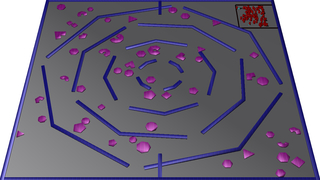
\includegraphics[width=0.24\textwidth]{usef/figC_Inter4_scaled.jpg}\\[2mm]
(c) scene 3
\caption{Illustration of $\Name$ on three different scenes. For each
  scene, several frames of a run of $\Name$ are shown. The first frame shows the
  swarm in the initial placement. The last frame shows the swarm when
  each robot has reached the goal region. The other frames show how the
  swarm progresses towards the goal region. Guides, which are computed
  by searching the roadmap, are shown in green arrows. Note that
  $\Name$ uses alternative guides when necessary to avoid collision with
  dynamic obstacles.}
\label{fig:ResQual}
\end{figure*}


\subsection{Experimental Setup}

An illustration of the three different scenes used in the experiments
is provided in Fig.~\ref{fig:Scenes}. Each scene is comprised of
static and dynamic obstacles. These scenes provide challenging test
cases as the swarm has to go through numerous narrow passages that are
frequently blocked by the random motions of the dynamic obstacles.


\subsubsection{Random Motions for the Dynamic Obstacles} Recall that $\Name$
has no \emph{a priori} information on the behavior of the dynamic obstacles. In
the experiments, the dynamic obstacles are made to move at random. More
specifically, each dynamic obstacle moves in small steps toward a random point.
When it reaches the random point or encounters a static or a dynamic obstacle,
it starts moving toward another random point. The dynamic obstacles move about
2--4 times slower than the robots.

The initial placement of the dynamic obstacles is also done at
random. More specifically, the $i$-th dynamic obstacle $o_i$ is placed
by generating a random position inside $W$ repeatedly until the
placement of $o_i$ is not in collision with the static obstacles, the
previously-placed dynamic obstacles $o_1, \ldots, o_{i-1}$, and the
robots in their initial placement.



\begin{figure}
\centering
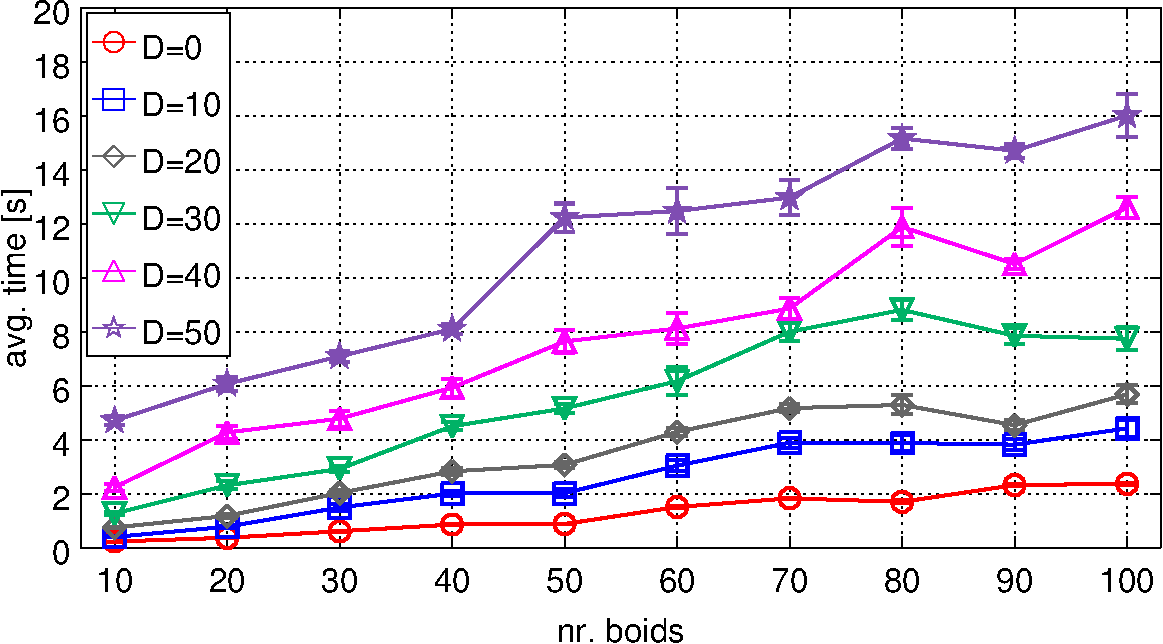
\includegraphics[width=\columnwidth]{usef/figResDynamicA}\\
(a) results for scene 1 \\
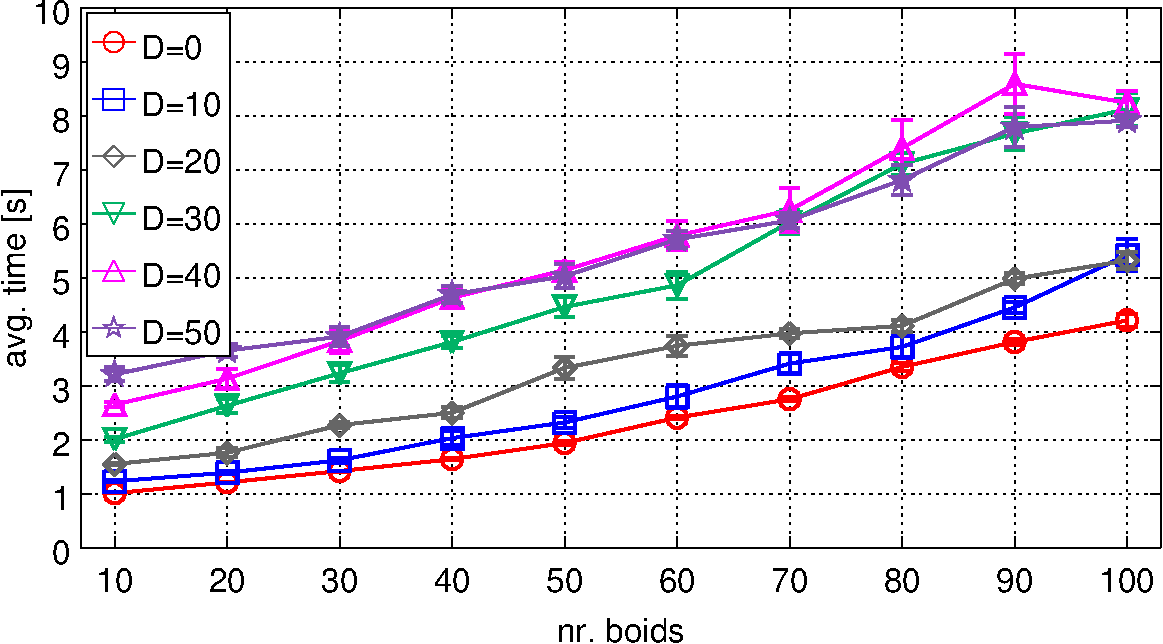
\includegraphics[width=\columnwidth]{usef/figResDynamicB}\\
(b) results for scene 2\\
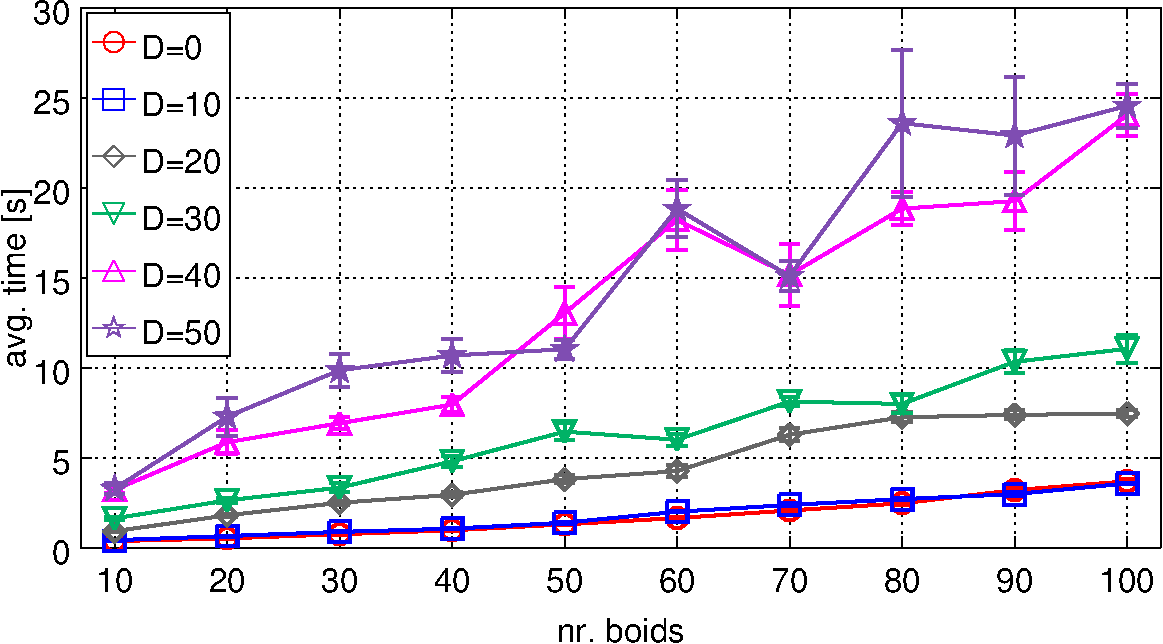
\includegraphics[width=\columnwidth]{usef/figResDynamicC}\\
(c) results for scene 3
\caption{Results show the mean runtime and standard deviation as a
  function of the number of robots and the number ($D$) of dynamic obstacles
  Runtime is measured as the time
  from the beginning till the last robot reaches the goal. It also
  includes the time to construct the roadmap (around 0.2s, roadmap
  used $n=5000$ vertices and $k=15$ neighbors). Mean is
  computed over twenty different runs for each problem instance. }
\label{fig:Res1}
\end{figure}




\subsubsection{Measuring Performance}
A problem instance is defined by a scene, the number of robots, and
the number of dynamic obstacles. In the experiments, the number of
robots is varied from $10$ to $100$ in increments of $10$. The number
of dynamic obstacles is varied from $0$ to $50$ in increments of
$10$.  Results for each
problem instance report mean time and standard deviation based on
twenty different runs. Runtime includes the time to construct the
roadmap, which was negligble (around 0.2s).  Experiments are conducted on an
Intel Core i7 machine (CPU: 2.40GHz, RAM: 8GB) using Ubuntu 14.04. Code is
written in C++ and compiled with g++4.8.2 using the optimization flag O2.

\subsection{Results}
\label{sec:Results}

Fig.~\ref{fig:ResQual} provides snapshots of $\Name$ when run on the
three different scenes. These snapshots show that the swarm reaches
the goal region, making use of alternative guides at times in order to
avoid the obstacles. As shown next, $\Name$ is quite efficient and the
running time scales linearly with the number of robots.

\subsubsection{Scalability as a Function of the Number of Robots and Dynamic
  Obstacles} Fig.~\ref{fig:Res1} provides a summary of the results
when varying both the number of the robots and the number of the
dynamic obstacles.  These results show that $\Name$ is capable of
efficiently enabling the swarm to reach the final goal while avoiding
collisions with static and dynamic obstacles. The third scene presents
the most challenging test case as the motions of the dynamic obstacles
often block the small openings through which the swarm needs to pass
in order to reach the goal region. As the results indicate, in all
scenes, $\Name$ scales linearly with the number of robots, even as the
number of the dynamic obstacles is increased.  By combining roadmaps
with potential fields, $\Name$ provides the swarm with global path
planning to guide the robots toward the goal region while reacting to
obstacles encountered along the way, making local adjustment and
seeking alternative guides to avoid getting trapped.

\subsubsection{Impact of Roadmap}

Results in Fig.~\ref{fig:ResPRMnv} and \ref{fig:ResPRMnn} show the
impact of the roadmap on the overall performance of $\Name$.
Fig.~\ref{fig:ResPRMnv} provides a summary of the results when varying
the number of roadmap vertices ($n$ in Alg.~\ref{algo:PRM}). In the
case of scenes 1 and 2, even roadmaps with a small number of vertices
are able to capture the connectivity of the free space and provide
viable pathways to guide the swarm. In these cases, $\Name$ performs
better with smaller roadmaps as it saves on the computational time
required to query the roadmap to compute the robot guides without
sacrificing the quality of the guides. In the case of scene 3, which
provides a more challenging environment, the smaller roadmaps are not
able to capture the connectivity of the free space. As a result, the
quality of the guides deteriorates, which makes it more difficult for
the robots to reach the goal region.  Also, when the roadmap becomes
too large, the performance suffers from the computational cost
associated with guide computations. Although finding an optimal number
of roadmap vertices remains challenging
\cite{book:MP,IncrementalPRM,RRTStar}, results show that
$\Name$ works well for a wide range of values, e.g., $1000-5000$ for
scenes 1 and 2, and $2500-7500$ for scene 3. 


Fig.~\ref{fig:ResPRMnn} provides a summary of the results when varying
the number of nearest neighbors ($k$ in Alg.~\ref{algo:PRM}) used for
the roadmap construction. These results show that $\Name$ works well
for a wide range of values. When $k$ becomes too large, there is an
increase in the running time of $\Name$ due to the larger
computational cost to query the roadmap. Also note that in the case of
scene 3, when $k$ is small, it becomes difficult to capture the
connectivity of the free space, which results in increased runtime for $\Name$
since the robot guides are not as effective.

\begin{figure}
\centering
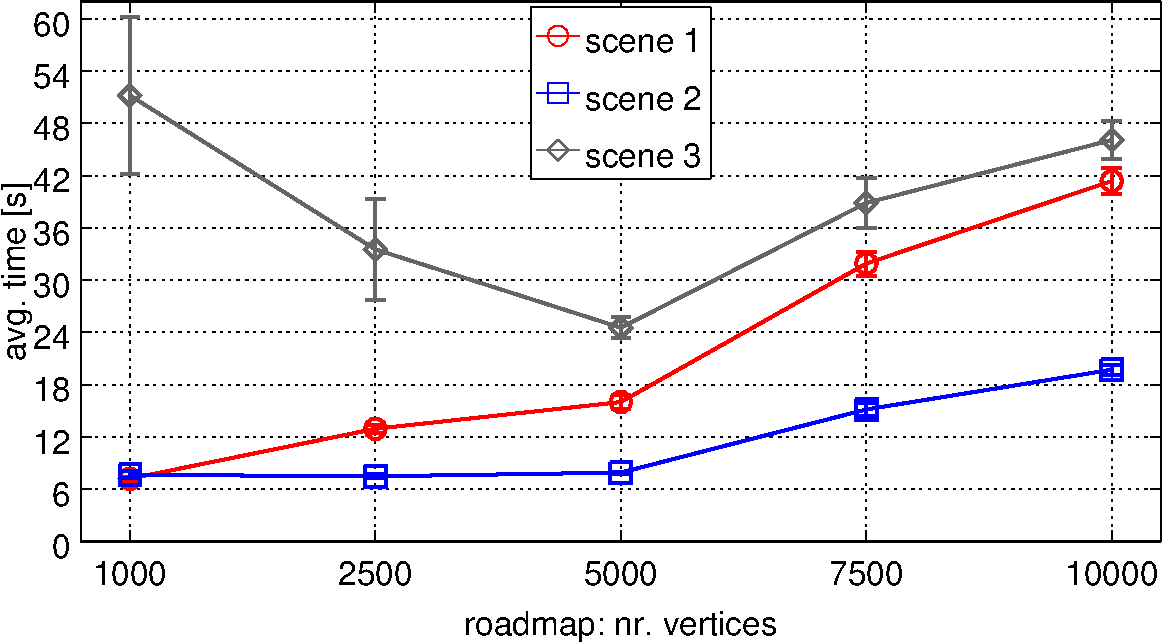
\includegraphics[width=0.8\columnwidth]{usef/figResPRMnv}
\caption{Results show the mean runtime and standard deviation as a
  function of the number of roadmap vertices ($n$ in
  Alg.~\ref{algo:PRM}).
  The number of nearest neighbors is kept at $k=15$. Results are shown for
  the case of 100 robots and 50 dynamic obstacles.  Runtime is measured
  as the time from the beginning till the last robot reaches the
  goal. Mean is computed over twenty different runs for each problem
  instance.}
\label{fig:ResPRMnv}
\end{figure}

\begin{figure}
\centering
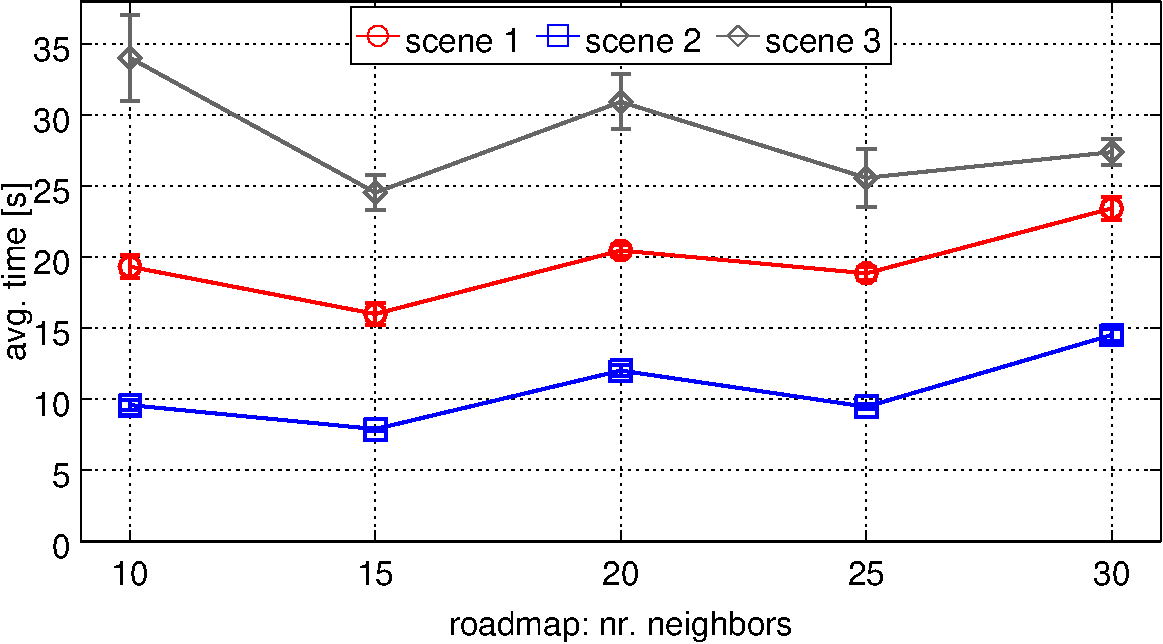
\includegraphics[width=0.8\columnwidth]{usef/figResPRMnn}
\caption{Results show the mean runtime and standard deviation as a
  function of the number of nearest neighbors ($k$ in
  Alg.~\ref{algo:PRM}) used for the roadmap construction.
  The number of   roadmap vertices is kept at $n=5000$. Results are shown for
  the case of 100 robots and 50 dynamic obstacles.  Runtime is measured
  as the time from the beginning till the last robot reaches the
  goal. Mean is computed over twenty different runs for each problem
  instance.}
\label{fig:ResPRMnn}
\end{figure}


\begin{figure*}
\centering
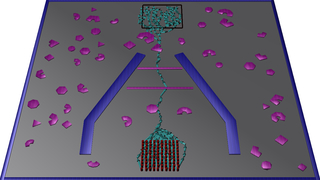
\includegraphics[width=0.19\textwidth]{usef/figDno_Inter1_scaled.jpg}
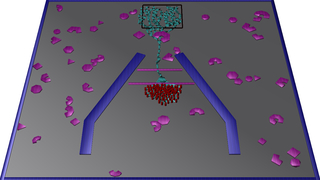
\includegraphics[width=0.19\textwidth]{usef/figDno_Inter2_scaled.jpg}
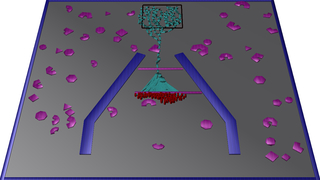
\includegraphics[width=0.19\textwidth]{usef/figDno_Inter3_scaled.jpg}
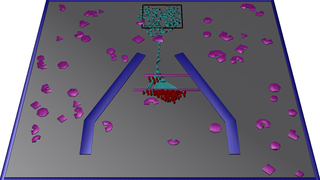
\includegraphics[width=0.19\textwidth]{usef/figDno_Inter4_scaled.jpg}
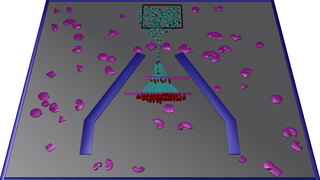
\includegraphics[width=0.19\textwidth]{usef/figDno_Inter5_scaled.jpg}\\
{\footnotesize{(a) $\Name$ with global replanning disabled}}\\[2mm]

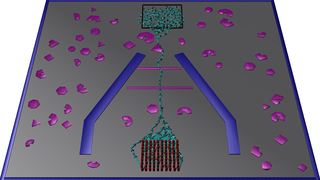
\includegraphics[width=0.19\textwidth]{usef/figD_Inter1_scaled.jpg}
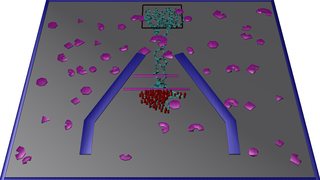
\includegraphics[width=0.19\textwidth]{usef/figD_Inter2_scaled.jpg}
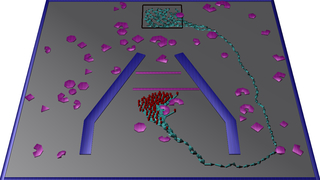
\includegraphics[width=0.19\textwidth]{usef/figD_Inter3_scaled.jpg}
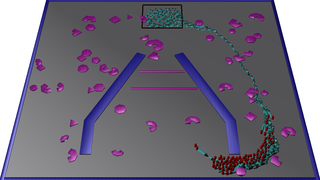
\includegraphics[width=0.19\textwidth]{usef/figD_Inter4_scaled.jpg}
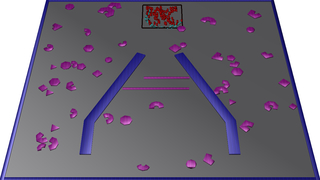
\includegraphics[width=0.19\textwidth]{usef/figD_Inter6_scaled.jpg}\\
{\footnotesize{(b) $\Name$ with global replanning enabled}}

\caption{Illustration of the importance of global replanning via
  alternative guides in $\Name$.
The thin, rectangular, dynamic obstacles, which move left and right and a
bit up and down, make it difficult for the swarm
to reach the goal by following the initial guide.
(a) When global replanning is disabled, the swarm gets stuck trying to pass
these obstacles by following the initial guide.
(b) When global replanning is enabled, once a robot become stuck,  an
alternative guide is computed, making it possible for the swarm to
effectively reach the goal region.}
\label{fig:ResBranch1}
\end{figure*}


\subsubsection{Impact of Global Replanning}



Fig.~\ref{fig:ResBranch1} provides a qualitative evaluation of the
impact of global replanning via alternative guides on the overall
performance of $\Name$. As shown, without global replanning, it 
becomes difficult for the swarm to find a way around the dynamic
obstacles which prevent the swarm from reaching the goal by
following the initial guide. With global replanning, the swarm can
make use of alternative pathways to reach the goal region.

Table~\ref{table:ResBranch2} shows the running time of $\Name$ when
global replanning is enabled vs disabled. As expected, $\Name$ fails
to find a solution when global replanning is disabled since the
dynamic obstacles prevent the swarm from reaching the goal. When
global replanning is enabled, $\Name$ efficiently guides the swarm to
the goal region by using alternative pathways.  This is because of two
things.  First, global replanning relieves the congestion around
narrow passageways and tries to split the swarm so it can ``move in
parallel.'' This means that instead of all of the robots going through
one passageway sequentially, two groups of robots can go through
different paths at the same time. The second reason global replanning
produces better results is because the robots are not able to
pre-generate a shortest path that will always keep the swarm out of
unrecoverable configurations as they do not posses the ability to
predict the position of dynamic obstacles.  When a dynamic
obstacle obstructs a narrow passageway and the shortest path goes
through that passageway, as in
Fig.~\ref{fig:ResBranch1}, without global replanning the robots will
not be able to reach the end until the obstacle moves out of the
way. With global replanning enabled, the swarm is able to find a new
way around the dynamic obstacle, therefore avoiding the obstructed
passageway. This reduces the amount of time the swarm spends waiting
and instead finds a new and more effective way to the goal region. 


\begin{table}
\centering
\begin{tabular}{c||r|r||r|r}
   & \multicolumn{2}{c||}{global replanning on} &
  \multicolumn{2}{c}{global replanning off}\\\hline
nr. robots & mean & std & mean & std\\
20 & 4.14s & 0.32 & x & x\\
40 & 5.66s & 0.32 & x & x\\
60 & 8.00s & 0.52 & x & x\\
80 & 10.70s & 0.82 & x & x\\
100 & 11.77s & 1.02 & x & x
\end{tabular}
\caption{Comparison of $\Name$ when global replanning is enabled vs
  disabled. Results are for the scene shown in
  Fig.~\ref{fig:ResBranch1}. Entries marked with x indicate that
  $\Name$ failed to find a solution in the allowed time of $120$s per
  run.}
\label{table:ResBranch2}
\end{table}

\section{Discussion}

This paper proposed $\Name$, a path-planning approach to enable a
swarm of robots move to a goal region while avoiding collisions with
static and dynamic obstacles. Scalability is obtained by an efficient
combination of probabilistic roadmaps to provide global path planning
with potential fields to provide local, reactive, behaviors necessary
to avoid collisions with obstacles. $\Name$ leverages past history and
global replanning via alternative guides to help stuck robots successfully find
their way to the goal. Experimental results with an increasing number
of robots and numerous dynamic obstacles show the efficiency and
scalability of the approach.  For future work, one direction is to
predict the motions of the dynamic obstacles and incorporate those
predictions to adjust the roadmap so that it can provide alternative
guides that avoid predicted trajectories. Improving the roadmap
quality could also improve the overall performance of $\Name$. Another
direction is to make use of high-level formation behaviors that can be
leveraged to more easily move through certain narrow passages.

\bibliographystyle{IEEEtran}
\bibliography{mp,plaku}


\end{document}

